\chapter{Results}\label{ch:results}

State parameters that were given, i.e. assimilation period, ensemble size.

\begin{figure}[h]
    \centering
    \begin{subfigure}[h]{0.4\textwidth}
        \includegraphics[width=\textwidth]{before_update_100}
        \caption{Before update.}
        \label{fig:abm_before}
    \end{subfigure}
    ~
    \begin{subfigure}[h]{0.4\textwidth}
        \includegraphics[width=\textwidth]{after_update_100}
        \caption{After update.}
        \label{fig:abm_after}
    \end{subfigure}
    \caption{Effect of Kalman Filter update on state of ABM.}
    \label{fig:enkf_abm}
\end{figure}

\begin{figure}[h]
    \centering
    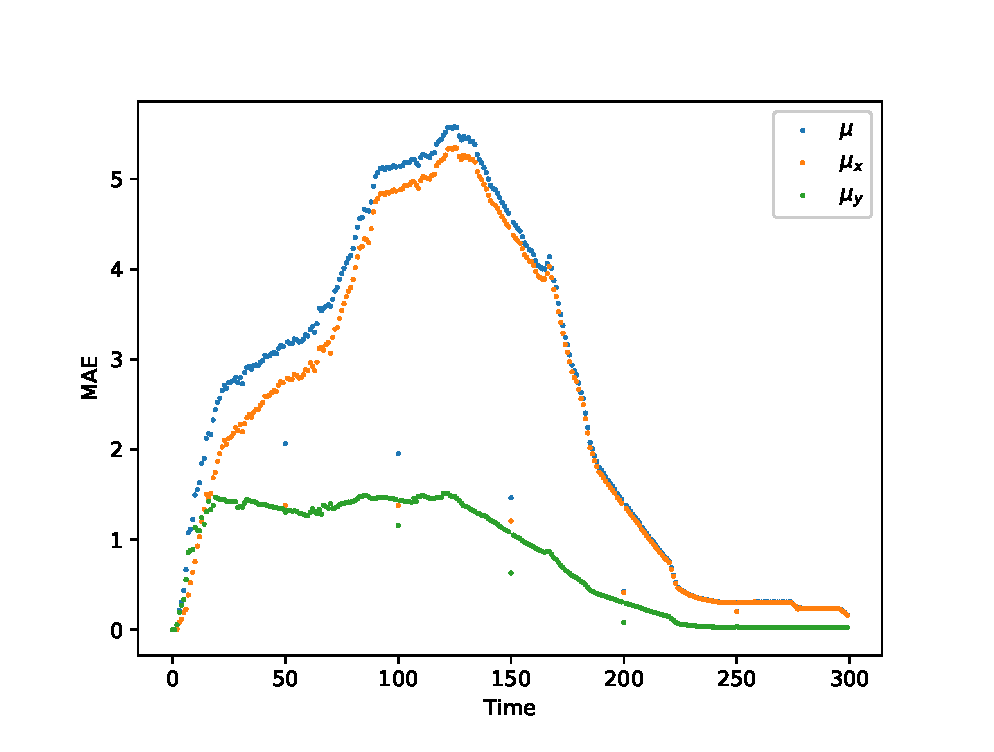
\includegraphics[width=0.8\textwidth]{errors}
    \caption{Variation of errors with simulation time.}
    \label{fig:errors}
\end{figure}
